\section{Fitting Procedures and Errors}\label{appFitting}

\textbf{
    In this section we give more details on how we compute the VSFs and their scaling parameters.
    As described in Sect.~\ref{methods:vsf} our previous discussions are based on VSFs that are computed from average relative velocities. 
    This means the following:
}

\textbf{ 
    We map the 3D FLASH data of the original simulations \citepalias{IbanezMejia2016} onto data cubes. 
    Those cubes consists of 400$^3$ subcubes, each representing a volume of (0.1~pc)$^3$, with the centre of the cubes being close to the centres of the molecular clouds. 
}

\textbf{
    As a consequence, we can only offer a discrete representation of the velocity information. 
    No matter whether a density threshold is applied or not, this binning still represents an amount of data that is computationally hard to process.
    For deriving and analysing the VSFs we coarsen the grid of projected lag distances, $\ell_i = |\vec{\ell}|_i$, so that separates the range between 0.1 and 30~pc into only 40 equidistant bins.
}

\textbf{
    Going back to the simulated data we apply two approaches: 
    The first strategy considers the density threshold, n$_\mathrm{cloud}$.
    This means that we pick only those cells from the data cubes that contain number densities equal to or larger than n$_\mathrm{cloud}$.
    These cells represent the starting points $\vec{x}$ (see Eqs.~\ref{equ:method:def_vsf}--\ref{equ:method:def_vsf_1d}).
    Our routine goes to each of these cells and calculated the lag distance to every other cell in the sample, as well as the relative velocities of the gas that is simulated within the given cells. 
    The individual lag distances are summarised into spherical shells around the starting points that range from inner radii $\ell_{i}$ to outer radii $\ell_{i+1}$. 
    By doing so, we compute the discrete VSFs presented in the main part of this paper with the relative velocities and product of densities, $\rho(\vec{x}) \cdot \rho(\vec{x}+\vec{\ell})$, measured from cells within the individual shells.
}

\textbf{
    The second approach targets the case when we do not apply any density threshold, or setting n$_\mathrm{cloud}$~=~0.
    In this case, we use python's random number generator \rc{!!! name of package !!!} to generate a set of cells within the entire data cubes that reflect 5\% of the total volume. 
    Thereby, we check that there are no duplicates within the sample.
    The so generated set of starting point is used for the analysis.
    As it is too computationally expensive to derive all relative velocities between all cells with the discrete shells, as we have done in the first approach, we derived a discrete distribution of relative velocities as function of lag distance using the Discrete Fast-Fourier-Transformation (\texttt{FFT}) offered by python.
    These distributions are based on the same grid of lag distances we have already utilised for the spherical shells above.
    Therefore, we can use the results of the \texttt{FFT} in the same way as the results from the first approach to derive the VSFs.
}

\textbf{
    With both approaches we obtain a set of discrete descriptions of VSFs as function of time (as the routines have been applied for all snapshots) and lag distance (which is identical with the grid of lag distances we have introduced above).
    In order to derive the scaling parameters, $\zeta$, of the VSFs as function of time and order, we use python's \texttt{curve\_fit} package to fit the power-law relation presented in Eq.~\ref{equ:method:fitting} to the measured VSFs.
    Due to the rather irregular behaviour of our VSFs at larger scales, we define the weighting function in such a way that is emphasis the inner region of clouds, $\ell\,\leq$~8~pc, and ceases outside with 1~pc/$\ell$[pc]. 
    \rc{!!! check !!!}
}

\textbf{
    Although the average radii of our clouds are, on average, larger than 8~pc we choose this limit due the variable behaviour of the VSFs at the edges of the clouds. 
    As can be seen in Fig.~\ref{pic:results:vsf_example}, as well as in the figures shown in Appendix~\ref{appFigures} the shape of VSFs changes over time, or better according to the interactions with the acting forces.
    Neither SNe blast waves nor gravitational contraction are able to act on all scales of the clouds simultaneously. 
    Instead, the shocks and accelerations propagate through the clouds at affect different parts of the clouds at different times.
    This is reflected in the evolution of VSFs, as well.
    For example, when a shock front, produced during a SN explosion, impacts one of the clouds, it does not compress all the cloud's gas at the same time.
    Rather it compresses the matter within a segment at edge of the cloud that is closest to the SN site.
    From there on, the shock propagates through the cloud.
    Yet, by the time when the shock front reaches the far end of the cloud the closer end, where the interaction between blast wave and cloud has started, relaxes already; within a short period of time as our observations in Sect.~\ref{results} show.
    In terms of VSF this scenario the described scenario means the following:
    In the first step, when the blast wave shocks the cloud first, the values of $S_\mathrm{p}$ increases at large lag scales first.
    This is because of the distribution of cells belonging to the cloud. 
    As the density of the cloud increases forwards the centre of the cloud, there is a higher number of cells closer to the centre than to the edges. 
    Due to the way the VSF is defined (Eq.~\ref{equ:method:def_vsf}) this kind of distribution causes that the VSF at small $\ell$ is dominated by inner-cloud cells (with high densities and close distances to each others), while the outer regions of the cloud dominate the VSF at large values of $\ell$ (low densities and large separations).
    As the shock front propagates through the cloud, the values of $S_\mathrm{p}$ at all ranges of $\ell$ are amplified, yet the effect is strongest within the regions through which the shock is propagating.
}

\textbf{
    The similarity parameters, $Z$, are computed by applying Eq.~\ref{equ:method:z_def} on the results of the fitting procedure, and all results are presented in Sect.~\ref{results}.
}

\begin{figure*}
    \centering
    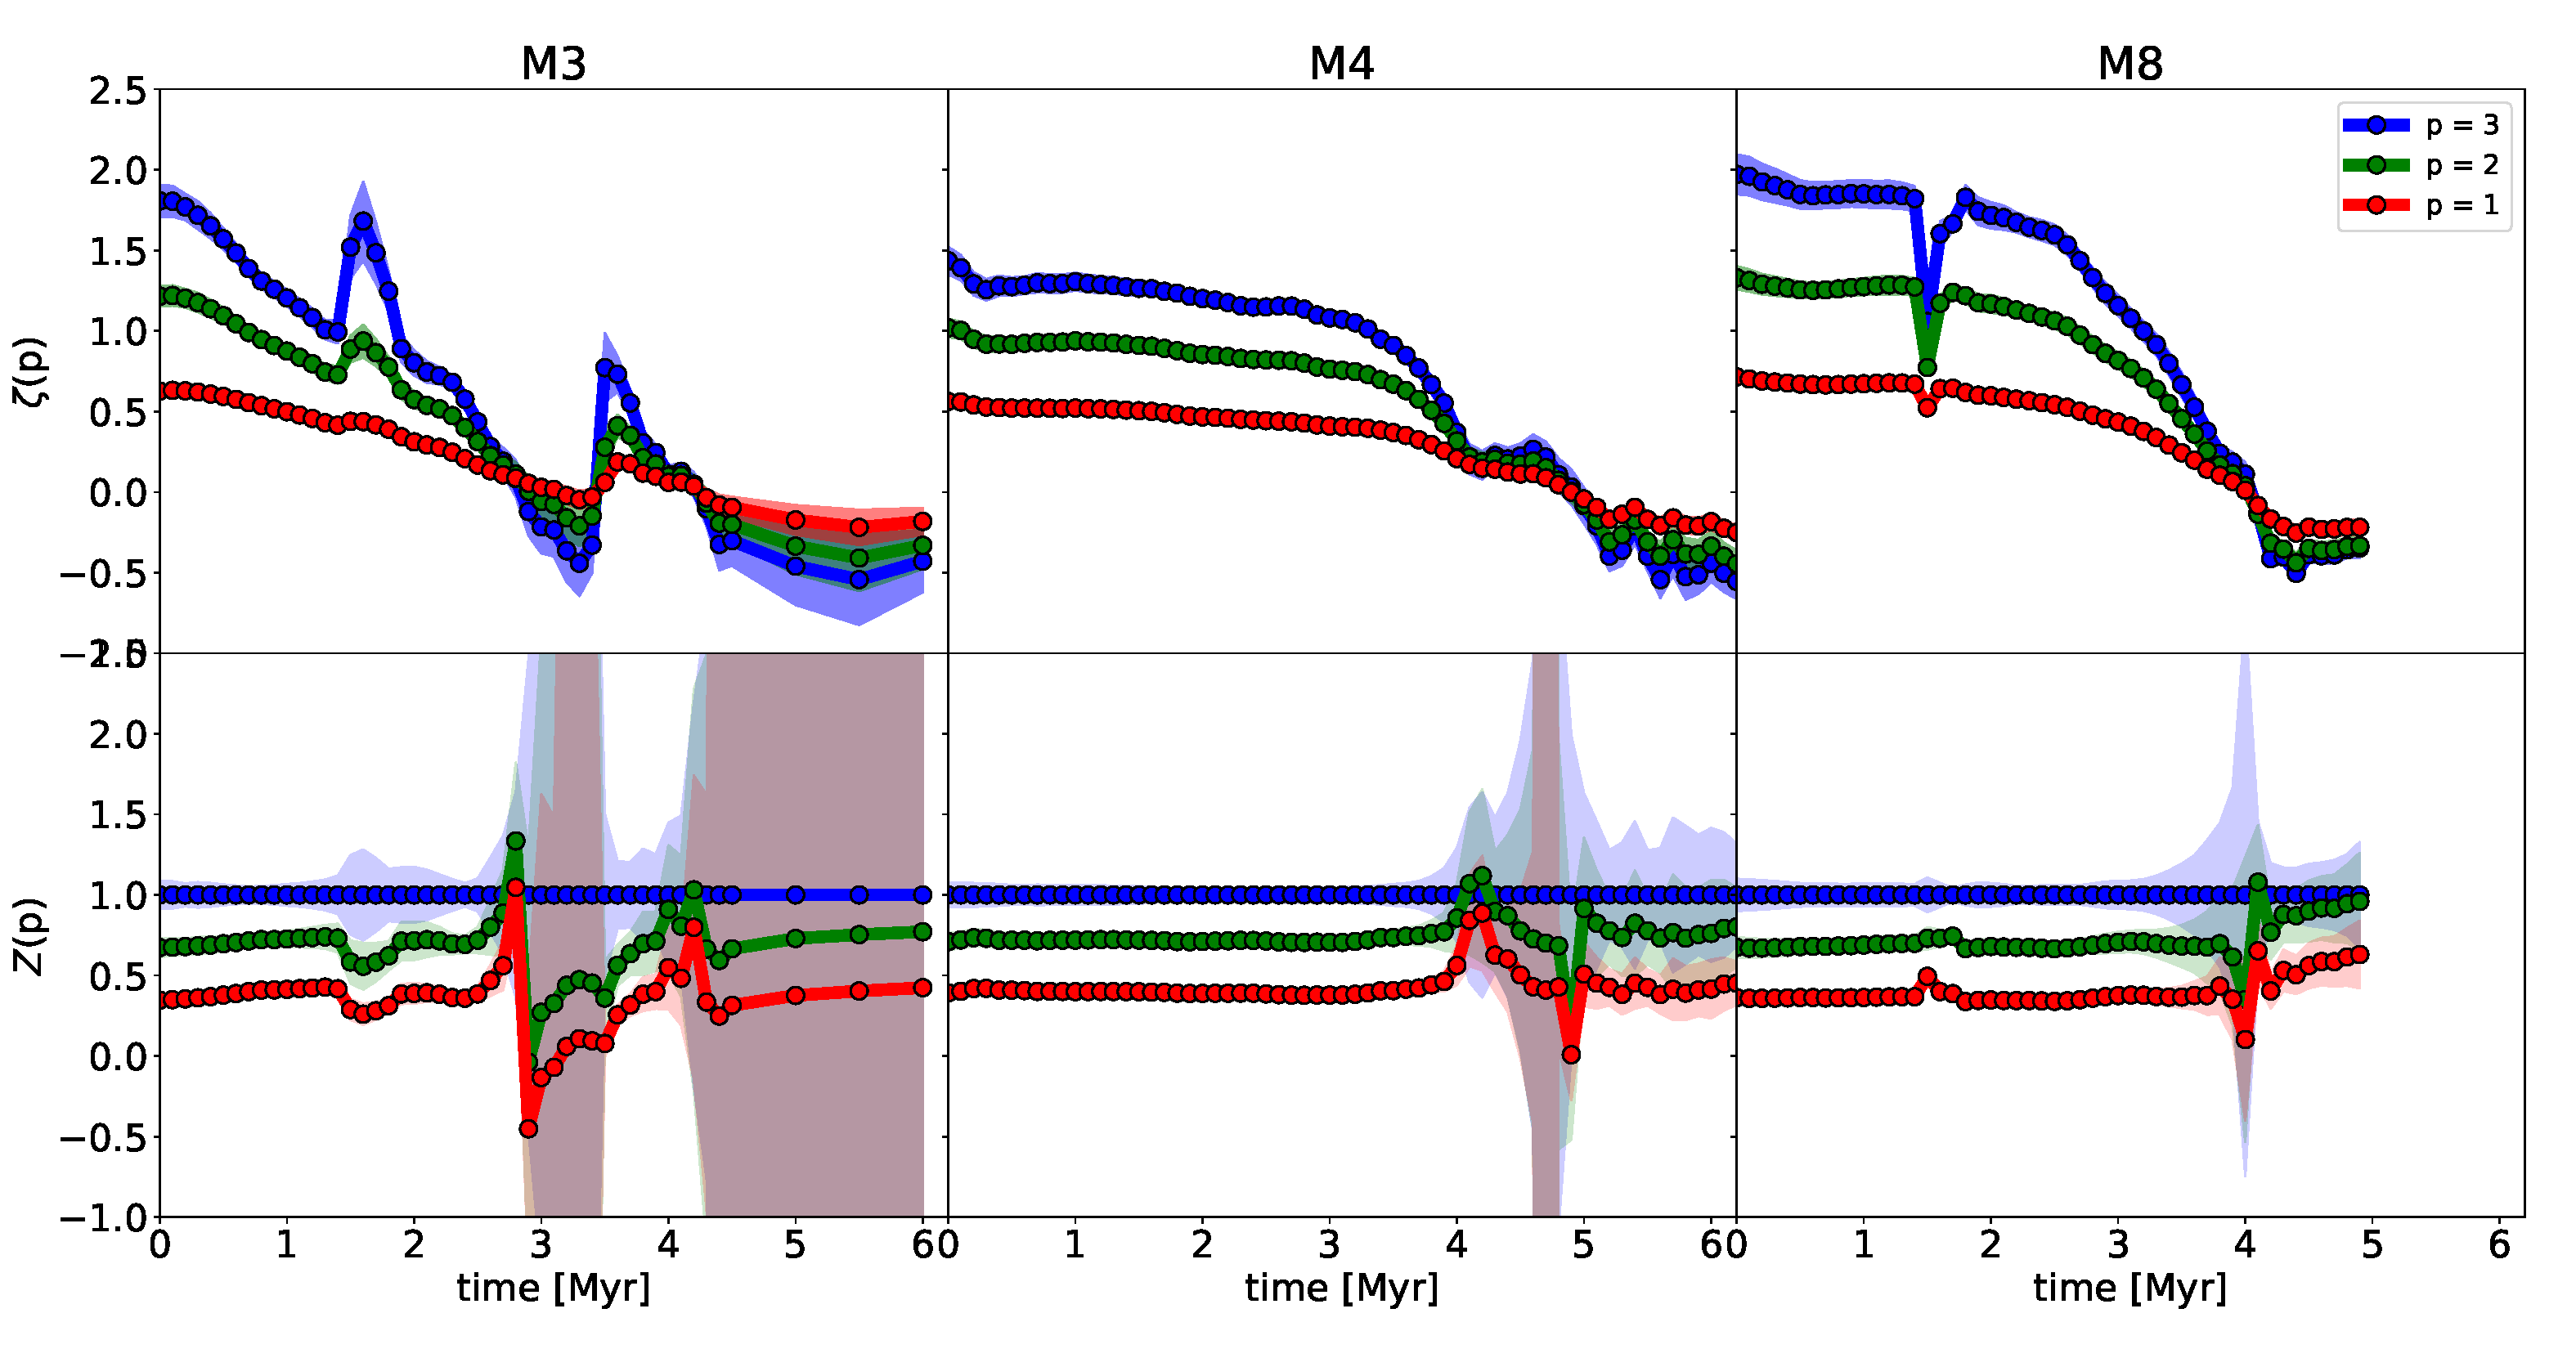
\includegraphics[width=\textwidth]{error_vsf04_zeta_z.pdf}
    \caption{
        Like Fig.~\ref{pic:results:zeta_all}a.
        Additionally, the shaded areas behind the data represent the error ranges of computed $\zeta$ (\textit{top}) and $Z$ (\textit{bottom}), respectively. 
    }
    \label{pic:appFitting:error_vsfhr04_zeta_z}
\end{figure*}


\textbf{
    From \texttt{curve\_fit} we also obtain the $\chi^2$ errors for measured $\zeta$. 
    In Fig.~\ref{pic:appFitting:error_vsfhr04_zeta_z} we show a reduced version of Fig.~\ref{pic:results:zeta_all}(a).
    This means that we only plot the time evolution of $\zeta$ for all three clouds.
    Additionally, we added shades of the same colours of the respective lines that represent the error areas as derived by \texttt{curve\_fit}.
    We see that the relative errors, $\Delta \zeta / \zeta$, are mostly within a range of 5--12\%. 
    Only when $\zeta$ becomes very negative, the errors increase as it is harder to unify the fall in $S_\mathrm{p}$ with larger $\ell$ with the requirement that $S_\mathrm{p} (\ell=0)$~=~0 (as there is no relative velocity measurable within one cell).
}

\textbf{
    The errors of $Z$ are computed by the Gaussian error propagation, given by:
}
\begin{align}\Delta Z(p) &= \sqrt{ \left( \frac{\partial Z(p)}{\partial \zeta(p)} \cdot \Delta\zeta(p) \right)^2 + \left( \frac{\partial Z(p)}{\partial \zeta(3)} \cdot \Delta\zeta(3) \right)^2 } \\
        &= \sqrt{ \left( \frac{\Delta\zeta(p)}{\zeta(3)} \right)^2 + \left( \frac{ \zeta(p) \cdot \Delta\zeta(3)}{\zeta(3)^2} \right)^2 }.
        \label{equ:appFitting:z_error}
\end{align}
\textbf{
    In general, the relative errors of $Z$ are, as well, around 10\%.
    Yet, we see exceptions with very large errors. 
    The reason for this is that at these times $\zeta$(3) is either equal to 0 or very close to it, which causes Eq.~\ref{equ:appFitting:z_error} to diverge.
}

\textbf{
    The codes for both deriving the VSFs, computing the scaling parameters, as well as for creating the figures of this manuscript are accessible via: \newline
    {\url{https://doi.org/10.5531/sd.astro.3}}.
}


\endinput
